\begin{figure}[h]
	\centering
	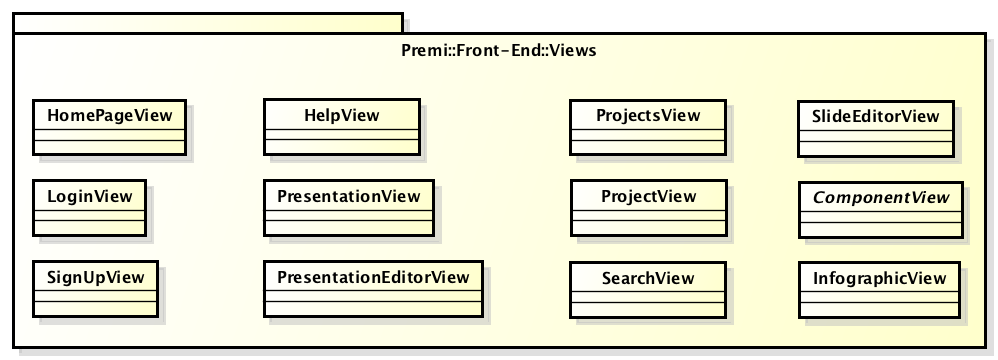
\includegraphics[width=0.7\linewidth]{img/premi_front_end_views}
	\caption[Premi::Front-End::Views]{Premi::Front-End::Views}
\end{figure}
Il package gestisce le view del front-end dell'applicazione. Comunica con il model, il controller e le direttive della struttura per acquisire i dati da visualizzare e far ottenere al model i dati modificati dall'utente attraverso il controller. Il package inoltre comunica con i framework esterni necessari per la creazione degli oggetti da utilizzare nel programma.

\subsubsection{ComponentView}
	\begin{figure}[h]
		\centering
		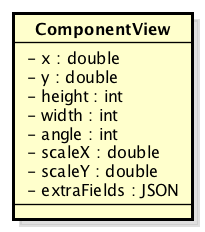
\includegraphics[width=0.4\linewidth]{img/premi_front_end_views_componentview}
		\caption[Premi::Front-End::Views::ComponentView]{Premi::Front-End::Views::ComponentView}
	\end{figure}
	
	\paragraph{Descrizione}
	ComponentView è la view che contiene i componenti che è possibile inserire in una slide e le rispettive informazioni.
	
	\paragraph{Utilizzo}
	Viene utilizzata come view per visualizzare e modificare gli attributi di un componente della slide.
	
	\paragraph{Relazioni con altre classi}
	\begin{itemize}
		\item \textbf{\textit{IN} componentController}:\\
		Classe che gestisce le operazioni e la logica applicativa riguardante la visualizzazione di un componente.
		\item \textbf{\textit{IN} slideEditorController}:\\
		Classe che gestisce le operazioni e la logica applicativa riguardante la visualizzazione e la modifica di una slide.
		\item \textbf{\textit{OUT} slideEditorView}:\\
		Classe che gestisce la visualizzazione e la modifica di una slide.
	\end{itemize}
	
	\paragraph{Attributi}
	\begin{itemize}
		\item \textbf{+ x: double}:\\
		Campo dati che contiene la coordinata x di origine del componente;
		\item \textbf{+ y: double}:\\
		Campo dati che contiene la coordinata y di origine del componente;
		\item \textbf{+ height: int}:\\
		Campo dati che contiene la l'altezza del componente;
		\item \textbf{+ width: int}:\\
		Campo dati che contiene la larghezza del componente;
		\item \textbf{+ angle: int}:\\
		Campo dati che contiene l'angolo di rotazione del componente;
		\item \textbf{+ scaleX: duble}:\\
		Campo dati che contiene la scala sull'asse x del componente;
		\item \textbf{+ scaleY: double}:\\
		Campo dati che contiene la scala sull'asse y del componente;
		\item \textbf{+ extraFields: JSON}:\\
		Campo dati che contiene un array JSON avente tutti i campi dati secondari di un componente;
	\end{itemize}


\subsubsection{HelpView}
	\begin{figure}[h]
		\centering
		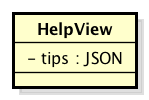
\includegraphics[width=0.4\linewidth]{img/premi_front_end_views_helpview}
		\caption[Premi::Front-End::Views::HelpView]{Premi::Front-End::Views::HelpView}
	\end{figure}
	
	\paragraph{Descrizione}
	È la view che contiene la parte di aiuto all'utente.
	
	\paragraph{Utiizzo}
	Viene utilizzata come view per visualizzare l'help.
	
	\paragraph{Relazioni con le altre classi}
	\begin{itemize}
		\item \textbf{\textit{IN} helpController}:\\
		Classe che gestisce la visualizzazione dell'aiuto all'utente.
	\end{itemize}
	
	\paragraph{Attributi}
	\begin{itemize}
		\item \textbf{+ tips:JSON}: \\
		Campo dati che contiene un array JSON con tutti gli aiuti da fornire all'utente.
	\end{itemize}
	
	
\subsubsection{HomePageView}
	\begin{figure}[h]
		\centering
		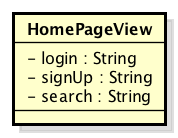
\includegraphics[width=0.4\linewidth]{img/premi_front_end_views_homepageview}
		\caption[Premi::Front-End::Views::HomePageView]{Premi::Front-End::Views::HomePageView}
	\end{figure}
	
	\paragraph{Descrizione}
	È la view che si occupa della gestione della pagina principale dell'applicazione.
	
	\paragraph{Utiizzo}
	Viene utilizzata come view per accedere alle principali sezioni dell'applicazione.
	
	\paragraph{Relazioni con le altre classi}
	\begin{itemize}
		\item \textbf{\textit{OUT} searchView}:\\
		Classe che gestisce la visualizzazione della ricerca nell'applicazione;
	\end{itemize}
	
	\paragraph{Attributi}
	\begin{itemize}
		\item \textbf{+ login: String}:\\
		Campo dati per il login di un utente all'applicazione;
		\item \textbf{+ signUp: String}:\\
		Campo dati per la registrazione di un utente all'applicazione;
		\item \textbf{+ search: String}:\\
		Campo dati per la ricerca nell'applicazione.
	\end{itemize}
	
	
\subsubsection{InfographicEditorView}
	\begin{figure}[h]
		\centering
		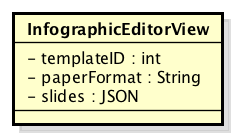
\includegraphics[width=0.4\linewidth]{img/premi_front_end_views_infographiceditorview}
		\caption[Premi::Front-End::Views::InfographicEditorView]{Premi::Front-End::Views::InfographicEditorView}
	\end{figure}
	
	\paragraph{Descrizione}
	È la view che si occupa della gestione della pagina relativa alle infografiche.
	
	\paragraph{Utiizzo}
	Viene utilizzata come view per visualizzare e creare le infografiche.
	
	\paragraph{Relazioni con le altre classi}
	\begin{itemize}
		\item \textbf{\textit{IN} infographicEditorController}:\\
		Classe che gestisce la visualizzazione delle infografiche e la loro creazione;
		\item \textbf{\textit{OUT} project}:\\
		Classe che gestisce un progetto e le sue componenti, cioè la presentazione e le infografiche.
	\end{itemize}
	
	\paragraph{Attributi}
	\begin{itemize}
		\item \textbf{+ templateId: int}:\\
		Campo dati per il template utilizzato dall'infografica;
		\item \textbf{+ paperFormat: String}:\\
		Campo dati per il formato adottato dall'infografica;
		\item \textbf{+ slides: JSON}:\\
		Campo dati contenente le slide incluse nell'infografica.
	\end{itemize}
	
	
\subsubsection{LoginView}
	\begin{figure}[h]
		\centering
		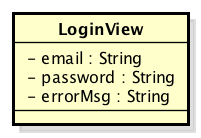
\includegraphics[width=0.4\linewidth]{img/premi_front_end_views_loginview}
		\caption[Premi::Front-End::Views::LoginView]{Premi::Front-End::Views::LoginView}
	\end{figure}
	
	\paragraph{Descrizione}
	È la view che si occupa della gestione della pagina relativa al login dell'utente al sito.
	
	\paragraph{Utiizzo}
	Viene utilizzata come view per autenticarsi all'applicazione.
	
	\paragraph{Relazioni con le altre classi}
	\begin{itemize}
		\item \textbf{\textit{IN} loginController}:\\
		Classe che gestisce l'autenticazione al sito;
		\item \textbf{\textit{OUT} projectsController}:\\
		Classe che gestisce la visualizzazione dell'account e dei progetti di un utente.
	\end{itemize}
	
	\paragraph{Attributi}
	\begin{itemize}
		\item \textbf{+ email: String}:\\
		Campo dati per l'email dell'utente;
		\item \textbf{+ password: String}:\\
		Campo dati per la password dell'utente;
		\item \textbf{+ errorMsg: String}:\\
		Campo dati contenente l'eventuale messaggio di errore da fornire all'utente.
	\end{itemize}
	
	
\subsubsection{PresentationEditorView}
	\begin{figure}[h]
		\centering
		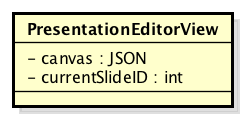
\includegraphics[width=0.4\linewidth]{img/premi_front_end_views_presentationeditorview}
		\caption[Premi::Front-End::Views::PresentationEditorView]{Premi::Front-End::Views::PresentationEditorView}
	\end{figure}
	
	\paragraph{Descrizione}
	È la view che si occupa della modifica di una presentazione.
	
	\paragraph{Utiizzo}
	Viene utilizzata come view per modificare una presentazione e le impostazioni generali di essa. Serve poi per accedere alla view per modificare la singola slide.
	
	\paragraph{Relazioni con le altre classi}
	\begin{itemize}
		\item \textbf{\textit{IN} presentationEditorController}:\\
		Classe che gestisce la modifica della presentazione;
		\item \textbf{\textit{OUT} slideEditorController}:\\
		Classe che gestisce la modifica di una slide.
	\end{itemize}
	
	\paragraph{Attributi}
	\begin{itemize}
		\item \textbf{+ canvas: JSON}:\\
		Campo dati che contiene un array JSON avente come elementi le slide della presentazione;
		\item \textbf{+ currentSlideId: int}:\\
		Campo dati che contiene l'id della slide corrente.
	\end{itemize}
	
	
\subsubsection{PresentationView}
	\begin{figure}[h]
		\centering
		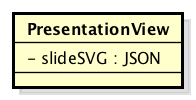
\includegraphics[width=0.4\linewidth]{img/premi_front_end_views_presentationview}
		\caption[Premi::Front-End::Views::PresentationView]{Premi::Front-End::Views::PresentationView}
	\end{figure}
	
	\paragraph{Descrizione}
	È la view che si occupa della visualizzazione di una presentazione.
	
	\paragraph{Utiizzo}
	Viene utilizzata come view per visualizzare e riprodurre la presentazione.
	
	\paragraph{Relazioni con le altre classi}
	\begin{itemize}
		\item \textbf{\textit{IN} presentationController}:\\
		Classe che gestisce la visualizzazione della presentazione.
	\end{itemize}
	
	\paragraph{Attributi}
	\begin{itemize}
		\item \textbf{+ slideSVG: JSON}:\\
		Campo dati che contiene un array JSON avente gli elementi in SVG per ogni slide della presentazione.
	\end{itemize}
	
	
\subsubsection{ProjectsView}
	\begin{figure}[h]
		\centering
		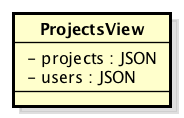
\includegraphics[width=0.4\linewidth]{img/premi_front_end_views_projectsview}
		\caption[Premi::Front-End::Views::ProjectsView]{Premi::Front-End::Views::ProjectsView}
	\end{figure}
	
	\paragraph{Descrizione}
	È la view che si occupa della gestione della pagina relativa all'utente e ai suoi progetti.
	
	\paragraph{Utiizzo}
	Viene utilizzata come view per visualizzare i dati dell'utente e accedere ai suoi progetti.
	
	\paragraph{Relazioni con le altre classi}
	\begin{itemize}
		\item \textbf{\textit{IN} projectsController}:\\
		Classe che gestisce la pagina dell'utente e dei suoi progetti;
		\item \textbf{\textit{OUT} infographic}:\\
		Classe che gestisce le infografiche di un progetto;
		\item \textbf{\textit{OUT} presentation}:\\
		Classe che gestisce la presentazione di un progetto.
	\end{itemize}
	
	\paragraph{Attributi}
	\begin{itemize}
		\item \textbf{+ projects: JSON}:\\
		Campo dati che contiene un array con i progetti dell'utente;
		\item \textbf{+ user: JSON}:\\
		Campo dati che contiene un array con i dati dell'utente.
	\end{itemize}
	
	
\subsubsection{ProjectView}
	\begin{figure}[h]
		\centering
		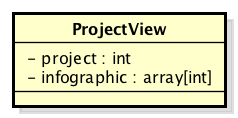
\includegraphics[width=0.4\linewidth]{img/premi_front_end_views_projectview}
		\caption[Premi::Front-End::Views::ProjectView]{Premi::Front-End::Views::ProjectView}
	\end{figure}
	
	\paragraph{Descrizione}
	È la view che si occupa della gestione di un progetto.
	
	\paragraph{Utiizzo}
	Viene utilizzata come view per visualizzare la presentazione e le infografiche di un progetto e per accedere alla sezione di modifica.
	
	\paragraph{Relazioni con le altre classi}
	\begin{itemize}
		\item \textbf{\textit{IN} projectController}:\\
		Classe che gestisce la pagina del progetto di utente;
		\item \textbf{\textit{OUT} presentationController}:\\
		Classe che gestisce la visualizzazione di una presentazione;
		\item \textbf{\textit{OUT} presentationEditorController}:\\
		Classe che gestisce la modifica di una presentazione;
		\item \textbf{\textit{OUT} infographicEditorController}:\\
		Classe che gestisce le infografiche e la loro modifica.
	\end{itemize}
	
	\paragraph{Attributi}
	\begin{itemize}
		\item \textbf{+ project: int}:\\
		Campo dati che contiene l'id della presentazione relativa al progetto;
		\item \textbf{+ infographic: [int]}:\\
		Campo dati che contiene un array con gli id delle infografiche relative al progetto.
	\end{itemize}
	

\subsubsection{SearchView}
	\begin{figure}[h]
		\centering
		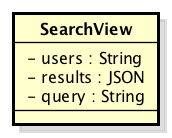
\includegraphics[width=0.4\linewidth]{img/premi_front_end_views_searchview}
		\caption[Premi::Front-End::Views::SearchView]{Premi::Front-End::Views::SearchView}
	\end{figure}
	
	\paragraph{Descrizione}
	È la view che si occupa della ricerca nell'applicazione.
	
	\paragraph{Utiizzo}
	Viene utilizzata come view per cercare un autore o un progetto nell'applicazione.
	
	\paragraph{Relazioni con le altre classi}
	\begin{itemize}
		\item \textbf{\textit{IN} searchController}:\\
		Classe che gestisce la ricerca nel sito;
		\item \textbf{\textit{IN} homePage}:\\
		Classe che gestisce la pagina principale dell'applicazione.
	\end{itemize}
	
	\paragraph{Attributi}
	\begin{itemize}
		\item \textbf{+ users: String}:\\
		Campo dati per identificare l'utente;
		\item \textbf{+ results: JSON}:\\
		Campo dati che contiene un array JSON con i risultati della ricerca;
		\item \textbf{+ query: String}:\\
		Campo dati contenente la query da eseguire per la ricerca.
	\end{itemize}
	
	
\subsubsection{SignUpView}
	\begin{figure}[h]
		\centering
		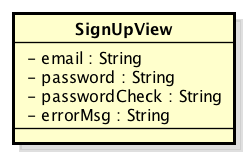
\includegraphics[width=0.4\linewidth]{img/premi_front_end_views_signupview}
		\caption[Premi::Front-End::Views::SignUpView]{Premi::Front-End::Views::SignUpView}
	\end{figure}
	
	\paragraph{Descrizione}
	È la view che si occupa della gestione della pagina relativa alla registrazione dell'utente al sito.
	
	\paragraph{Utiizzo}
	Viene utilizzata come view per registrarsi all'applicazione.
	
	\paragraph{Relazioni con le altre classi}
	\begin{itemize}
		\item \textbf{\textit{IN} signUpController}:\\
		Classe che gestisce la registrazione al sito;
		\item \textbf{\textit{OUT} loginController}:\\
		Classe che gestisce l'autenticazione dell'utente al sito.
	\end{itemize}
	
	\paragraph{Attributi}
	\begin{itemize}
		\item \textbf{+ email: String}:\\
		Campo dati per l'email dell'utente;
		\item \textbf{+ password: String}:\\
		Campo dati per la password dell'utente;
		\item \textbf{+ passwordCheck: String}:\\
		Campo dati per la ripetizione della password dell'utente;
		\item \textbf{+ errorMsg: String}:\\
		Campo dati contenente l'eventuale messaggio di errore da fornire all'utente.
	\end{itemize}
	
	
\subsubsection{SlideEditorView}
	\begin{figure}[h]
		\centering
		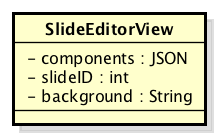
\includegraphics[width=0.4\linewidth]{img/premi_front_end_views_slideeditorview}
		\caption[Premi::Front-End::Views::SlideEditorView]{Premi::Front-End::Views::SlideEditorView}
	\end{figure}
	
	\paragraph{Descrizione}
	È la view che si occupa della modifica di una slide della presentazione.
	
	\paragraph{Utiizzo}
	Viene utilizzata come view per modificare una slide della presentazione, quindi per gestire gli elementi all'interno di essa.
	
	\paragraph{Relazioni con le altre classi}
	\begin{itemize}
		\item \textbf{\textit{IN} signUpController}:\\
		Classe che gestisce la registrazione al sito;
		\item \textbf{\textit{OUT} loginController}:\\
		Classe che gestisce l'autenticazione dell'utente al sito.
	\end{itemize}
	
	\paragraph{Attributi}
	\begin{itemize}
		\item \textbf{+ components: JSON}:\\
		Campo dati contenente un array con tutti gli elementi presenti nella slide;
		\item \textbf{+ slideId: int}:\\
		Campo dati per l'id delal slide corrente;
		\item \textbf{+ background: String}:\\
		Campo dati per il background della slidee.
	\end{itemize}